\documentclass[11pt,letterpaper]{article}

\usepackage{natbib}
%\usepackage{cite}
\usepackage{graphicx}
\usepackage[margin=1.in,centering]{geometry}
\usepackage{hyperref}
\usepackage{caption}
\usepackage[export]{adjustbox}
\usepackage{float}

\begin{document}

\title{Optical/UV Band
Reverberation Mapping of NGC 5548 with Frequency-Resolved Techniques}

\date{August 20, 2016}

\maketitle

\begin{abstract}

Power spectral densities and time lags of 19 wavelength bands are recovered as part of a reverberation mapping of NGC 5548. The latest time-variable light curves are made available in STORM III by \cite{2016ApJ...821...56F}. The uneven sampling of the data in those curves necessitates the use of a maximum likelihood method in conjunction with Fourier transformations to produce the frequency-dependent values of interest. This is the first time frequency-resolved time lags have been measured from UV/optical light curves in AGN. Variability in the emission is confirmed in the power spectral densities, and the time lags show a complex frequency dependence. The total power seen in each PSD decreases with wavelength, and the average time lag increases with wavelength, both in support of thermal reprocessing by an accretion disk. There are computational issues yet to be resolved regarding accurate error estimates, so errors presented here can only be considered a lower limit. The transfer function should be recoverable once those and any additional computational issues are resolved.

\end{abstract}


\section{Introduction}
\label{sec:intro}

Active galactic nuclei (AGN) are distant, powerfully luminous compact objects, with strongly variable spectra that have no recognized period. There is strong observational evidence that AGN influence galactic evolution through a process called AGN feedback (see \cite{2012ARA&A..50..455F} for a detailed review). Due to their immense luminosities, AGN are prime candidates to serve as standard candles by which to measure fundamental cosmological parameters -- well beyond the supernova horizon. The Hubble constant $H_0$ and deceleration parameter $q_0$ respectively describe the rate at which the universe is expanding and the rate at which gravity within the universe resists that expansion. \cite{1999MNRAS.302L..24C} presents a method for measuring these parameters by observing the wavelength-dependent time delays emergent from AGN systems, and this approach has been corroborated by \cite{2007MNRAS.380..669C}. Constraint of these parameters depends on properly modelling the light echo, or reverberation, effects within AGN. This work endeavors towards a better understanding of the accretion disk structure of AGN.

AGN systems are complex, with the widely-accepted picture having a super-massive black hole (SMBH) at the center, surrounded by an accretion disk, a much larger broad line region, an obscuring torus, and a relativistic matter jet. In almost all cases, astronomers are unable to resolve the configurations of these systems directly, because their angular size is far too small, so the geometry must be inferred using some other method. Reverberation mapping refers to the technique of inferring the configuration of a system by analysing the observed time lags between wavelength bands and recovering the transfer function which encodes the system geometry. It uses echoes of light to map the region surrounding the SMBH, analogous to mapping the sea floor using sonar. \cite{1999MNRAS.302L..24C} and \cite{2007MNRAS.380..669C} provide methods for constraining Hubble's constant and the deceleration parameter, with increasing certainty as the size of the dataset grows. While retaining sight of that ultimate goal, this work has a less-encompassing scope. The thermal reprocessing hypothesis describes the reprocessing of high-energy electromagnetic emission by the accretion disk; it is explained in greater detail in section \ref{sec:reverbmap}. The work executed herein attempts to test that hypothesis as one step toward greater understanding of the structure of AGN.  

The Type-I Seyfert galaxy NGC 5548 is one of the most studied Seyfert galaxies, and yet remains an object of intense interest. Seyfert galaxies are a subclass of AGN that are found in the local universe. The Space Telescope and Optical Reverberation Mapping Project (STORM) encompasses the most in-depth study of NGC 5548 yet performed \citep{2015ApJ...806..128D} \citep{2015ApJ...806..129E} \citep{2016ApJ...821...56F}. In part III of STORM, \cite{2016ApJ...821...56F} published the most complete set of time-dependent light curves yet collected for this object in the optical and UV spectrum. In section \ref{sec:reverbmap}, the theory of reverberation mapping is described in more detail, including details on using frequency-domain analyses to elucidate observed time delays between the wavelength bands, and determining the geometry of the system from the observed time delays by recovering the transfer function. In section \ref{analysis}, these methods are applied to the NGC 5548 light curves published in STORM III. Finally, the results are discussed in the context of whether they support the thermal reprocessing hypothesis.


\section{Reverberation Mapping}
\label{sec:reverbmap}

The standard hypothesis of reverberation mapping posits that high-energy photons from near the super-massive black hole at the center of an active galactic nucleus irradiate the surrounding matter which reprocesses the emission before it escapes toward the observer. If the propagation of these signals is assumed to travel at the speed of light, the geometry of the structures can be inferred from the observed time delays. Broad emission lines are thought to be reverberated responses to irradiation by the continuum, but this work focuses on reverberation in the accretion disk around the SMBH, i.e., the continuum emission, which is thought to respond thermally to irradiation by high-energy photons.

Reverberation mapping has become a standard technique for calculating the black hole masses of SMBH within AGN. This technique has been used to determine the masses of approximately 60 SMBH in AGN (see the \cite{2015PASP..127...67B} database for an up-to-date list). Reverberation mapping techniques are well-described by \cite{2014SSRv..183..253P}. They continue to be refined, and may also allow for measuring the spin of SMBH in AGN when applied to X-ray observations \citep{2016Natur.535..388K}. \cite{2007MNRAS.380..669C} and \cite{1999MNRAS.302L..24C} present similar methods for determining the distance to AGN using reverberation mapping. This Hubble's law-independent method for computing the distance to AGN provides an approach to recovering Hubble's constant and the deceleration parameter. However, the basic assumption of this method is that the structure of the accretion disk follows the standard \cite{1973A&A....24..337S} structure. This needs to be confirmed before accurate values can be constrained using Hubble's law. Initial results from \cite{2007MNRAS.380..669C} suggest that the accretion disks are larger than expected.

    \subsection{Continuum Reverberation}
    \label{sec:cont_reverb}
    
    The thermal reprocessing hypothesis suggests that a hot accretion disk is incident upon a central SMBH. High-energy EM emission, possibly in the form of X-rays, illuminate the disk, driving an increase in temperature in the disk that propagates at the speed of light. \cite{1999MNRAS.302L..24C} provide a model for the average expected time lag $\tau$ as a function of wavelength band $\lambda$, presented in equation \ref{eq:timelag}.

    \begin{equation}
        \label{eq:timelag}
        \tau\left(\lambda\right) = 
            \left(3.9 \textrm{d}\right) 
            \left(\frac{T_0}{10^4\mathrm{K}}\right)^{4/3}
            \left(\frac{\lambda}{10^4\mathrm{\AA}}\right)^{4/3}
            \left(\frac{X}{4}\right)^{4/3}
    \end{equation}

    This model assumes the accretion disk consists of a distribution of blackbody radiators with temperature distribution $T\left(R\right) = T_0\left(R/R_0\right)^{-3/4}$ with an irradiating source of high-energy emission along the axis of the disk at some height $H_0$ that is much larger than the height of the accretion disk $H$ ($H_0 \gg H$). $X$ represents a heuristic factor that comes out to $\sim3-4$ for blackbody radiation. Given some constant $X$, it can be seen from this model that $\tau \propto \lambda^{4/3}$. The temperature distribution predicts an increasing Wien wavelength in a positive radial direction, so the responding wavelengths should be longer as the source emission travels farther. Observing time lags that increase with wavelength will provide support for the thermal reprocessing hypothesis. Figure \ref{fig:disk_reverb} provides a very simple geometry of this process: high-energy emission emergent from the axis of the accretion disk illuminates and is reprocessed by the disk before escaping toward the observer.

    In the time domain, the correlated response curves at longer wavelengths are seen by inspection to be smeared. As the emission is reprocessed in the disk, it becomes blurred, so the variability can be expected to decrease with wavelength. Thus, the two main observational signatures of thermal reprocessing are that we expect that longer wavelength optical emission should be both lagged and less variable than UV emission. The exact relationship between wavelength and time lag will allow us to test the structure of the disk -- does it follow the $\tau \propto \lambda^{4/3}$ that is expected for a Shakura-Sunyaev disk?

    \begin{figure}
        \centering
        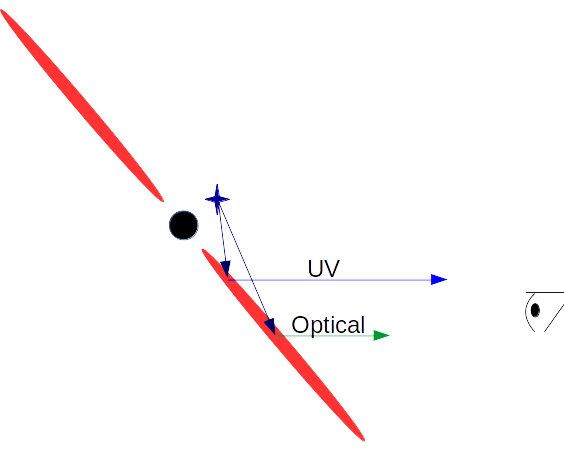
\includegraphics[width=2.5in]{../img/basic_geometry.png}
        \caption{Simple geometry of reverberation in the accretion disk. Some continuum emission is reprocessed before escaping toward the observer.}
        \label{fig:disk_reverb}
    \end{figure}


    \subsection{Frequency-domain Analysis}
    \label{sec:freq_analysis}

    The link between the driving and reprocessed light curves can be described using a transfer equation (equation \ref{eq:time_transfunc}). The reprocessed curve $y(t)$ is seen to be the convolution of the driving light curve $x(t)$ with a response function $g(t)$. The transfer function encodes the geometry of the system by describing the time-dependent response of the reverberated light curve relative to the reference curve for all wavelengths in the system. Recovering the function from the observed light curves is a primary goal of reverberation mapping and theoretically allows the reconstruction of the structures within an AGN. The convolution theorem provides that convolution in the time domain is equivalent to pointwise multiplication in the frequency domain (equation \ref{eq:freq_transfunc}). The transfer function therefore lends itself well to frequency-domain analyses.

    \begin{equation}
        \label{eq:time_transfunc}
        y(t) = \int_{-\infty}^{\infty} g(\tau) x(t-\tau)  {\rm d}\tau
    \end{equation}

    \begin{equation}
        \label{eq:freq_transfunc}
        Y(\nu) = G(\nu) X(\nu)
    \end{equation}

    The power spectral density (PSD) provides a measure of the variability of the flux in a band. It is defined as $|X(\nu)|^2 = X^*(\nu)X(\nu)$, where $^*$ denotes the complex conjugate, and can be produced using Fourier transforms. The response function is therefore related to the PSD of two light curves:

    \begin{equation}
        |Y(\nu)|^2 = |G(\nu)|^2 |X(\nu)|^2
    \end{equation}

    Given two bands, a cross spectrum can also be computed. The cross spectrum is defined as $C(\nu) = X^*(\nu) Y(\nu)$. The argument $\phi$ of the cross spectrum is the phase lag between the two signals. The time lag $\tau$ can therefore be computed from the cross spectrum using

    \begin{equation}
        \tau(\nu) = \frac{\phi(\nu)}{2\pi\nu}
    \end{equation}

    Given equation \ref{eq:freq_transfunc}, the cross spectrum can be written as

    \begin{equation}
        C(\nu) = X^*(\nu) G(\nu) X(\nu) =  G(\nu) |X(\nu)|^2
    \end{equation}

    The time lags are therefore trivially predicted as a function of frequency from the cross spectrum. The frequency dependence of these lags in turn relates directly to the transfer function. Very good explanations of these techniques and the associated mathematics are available from \cite{2014A&ARv..22...72U}.

    A tophat response function demonstrates these concepts. A tophat function provides a simple model of the time-dependent response of a delayed light curve for a single wavelength. A fast Fourier transform method provides the time lag spectrum (figure \ref{fig:th_freq}) for the tophat impulse response (figure \ref{fig:th_time}). Identifying some features can aid an intuitive understanding of time lag spectra of more complicated functions. In this simple case, the average time lag $\tau_0$ is shared across the frequency domain until $\nu=\frac{1}{2\tau_0}$, at which frequency the time lag phase wraps from $\pi$ to $-\pi$; in fact, this occurs at each interval of $\nu=\frac{n}{2\tau_0}$, with $n$ an odd integer. As the width of the time response function changes, i.e., the time response becomes more "smoothed out", the higher-frequency distribution of the time lag attenuates, but the wrapping frequency remains constant. \cite{2014A&ARv..22...72U} describes how even with dilution, the time lag distribution retains the feature, so this switching frequency can provide a measure of the average time lag from simple inspection. The time lag distribution can be recovered with a computational fit.

    Once the time lags are extracted from the observational datasets, they might be fitted with a tophat function, however, a more complicated function such as a log-Gaussian function is probably more appropriate, or physical models expected for an accretion can be tested too.

    \begin{figure}
        \centering
        \begin{minipage}{.475\textwidth}
            \centering
            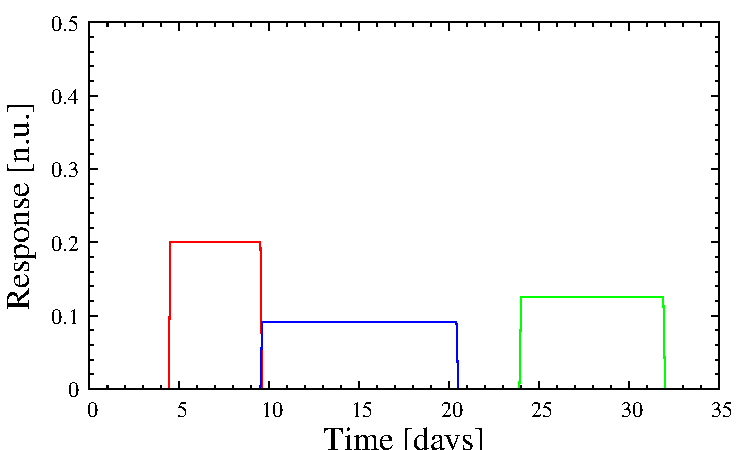
\includegraphics[width=1\linewidth]{../img/tophat_timedomain.pdf}
            \captionof{figure}{Tophat transfer functions in the time domain show an average time lag of the reverberating curve and a constant distribution in time over an interval. An area of unity indicates no loss of signal in the response.}
            \label{fig:th_time}
        \end{minipage}
        \hfill
        \begin{minipage}{.475\textwidth}
            \centering
            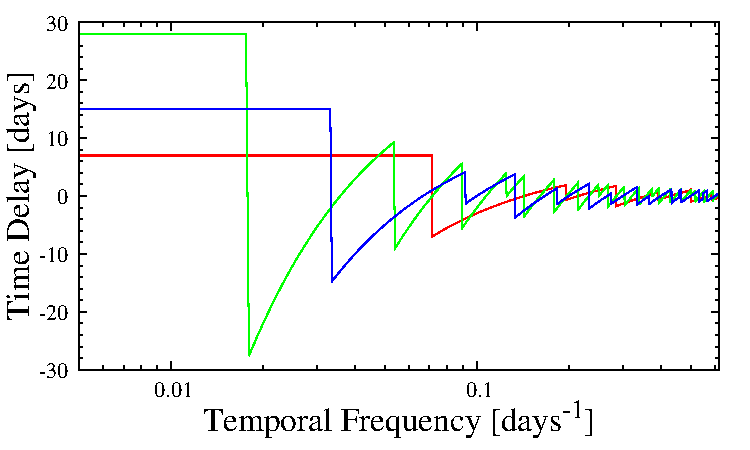
\includegraphics[width=1\linewidth]{../img/tophat_freqdomain.pdf}
            \captionof{figure}{The time lags associated with each tophat function. Distinct features related to the average time lag are present (maximum, value of $\nu$ at steepest change), and complicated relationships with higher frequency waves can be noted.}
            \label{fig:th_freq}
        \end{minipage}
    \end{figure}



	\subsection{Unevenly-Sampled Data}
    \label{sec:uneven_data}

    Traditional frequency-domain analyses require data that is evenly sampled. Due primarily to weather and other issues relating to scheduling observations on ground-based telescopes, optical reverberation mapping datasets generally have uneven sampling. Because of this, until now, optical reverberation mapping has been limited mainly to time-domain analyses, e.g., cross-correlation. Cross-correlation is useful to analyse datasets with significant sampling variability, but most analysis involving cross-correlation techniques ultimately recover the average lag only; however, more information is contained within the light curves than their average time lag.

    Some X-ray datasets contain gaps due to the approximately 90-minute orbital period for satellites in low-Earth orbit, which motivated the work by \cite{2013ApJ...777...24Z}, where a maximum likelihood method is used to perform the frequency-domain analyses prepared in section \ref{sec:freq_analysis} on light curves with gaps. Since its development, this technique has found success among studies of observations captured by low-orbit X-ray telescopes that exceed the telescopes' orbital periods, such as the analysis performed by \cite{2016Natur.535..388K}. For the first time, we are applying these techniques to UV/optical data, making use of the high-quality light curves published in STORM III. If successful, they may provide new insight into the reverberations present in the accretion disk and other structures of the nucleus in NGC 5548.

\section{Analysis of Light Curves in STORM III}
\label{analysis}
In part III of the Space Telescope and Optical Reverberation Mapping Project, \cite{2016ApJ...821...56F} published the best dynamic data yet collected from NGC 5548 over a 260-day period, for 19 bands throughout the optical and into the UV domains. They are presented in figure \ref{fig:lightcurves}. These data were collected from a variety of observatories, including space and ground-based facilities, and thus have significantly uneven and variable sampling rates. In STORM III, a reverberation mapping analysis is performed using cross-correlation to find the average time lag for each wavelength (figure \ref{fig:cc_analysis}). These results are superposed over some possible models and while lags increase with wavelength as expected from the the accretion disk model, the amplitude of the lags is about 10 times larger than expected based on the observed flux of the source, meaning that our understanding of accretion disk structure and/or reprocessing is incomplete. More information is contained in the light curves, so a frequency-domain analysis should provide better constraints.

The uneven sampling of these data suggest that the maximum likelihood method developed by \cite{2013ApJ...777...24Z} is a reasonable candidate for analysing them. Using the method described in section \ref{sec:uneven_data}, the power spectral densities and time lags as functions of temporal frequency are computed for each band in the dataset -- 18 bands not including the reference band. The 1367\AA$ $ light curve, obtained from observations made with the Hubble Space Telescope, is chosen as the reference curve. The power spectral density for 1367\AA$ $ is presented in figure \ref{fig:psd_1367}, giving a description of the flux variability seen in that band. Figure \ref{fig:timelag_7647} provides the time lag of variability observed at 7647\AA$ $ relative to 1367\AA$ $.

\begin{figure}
    \centering
    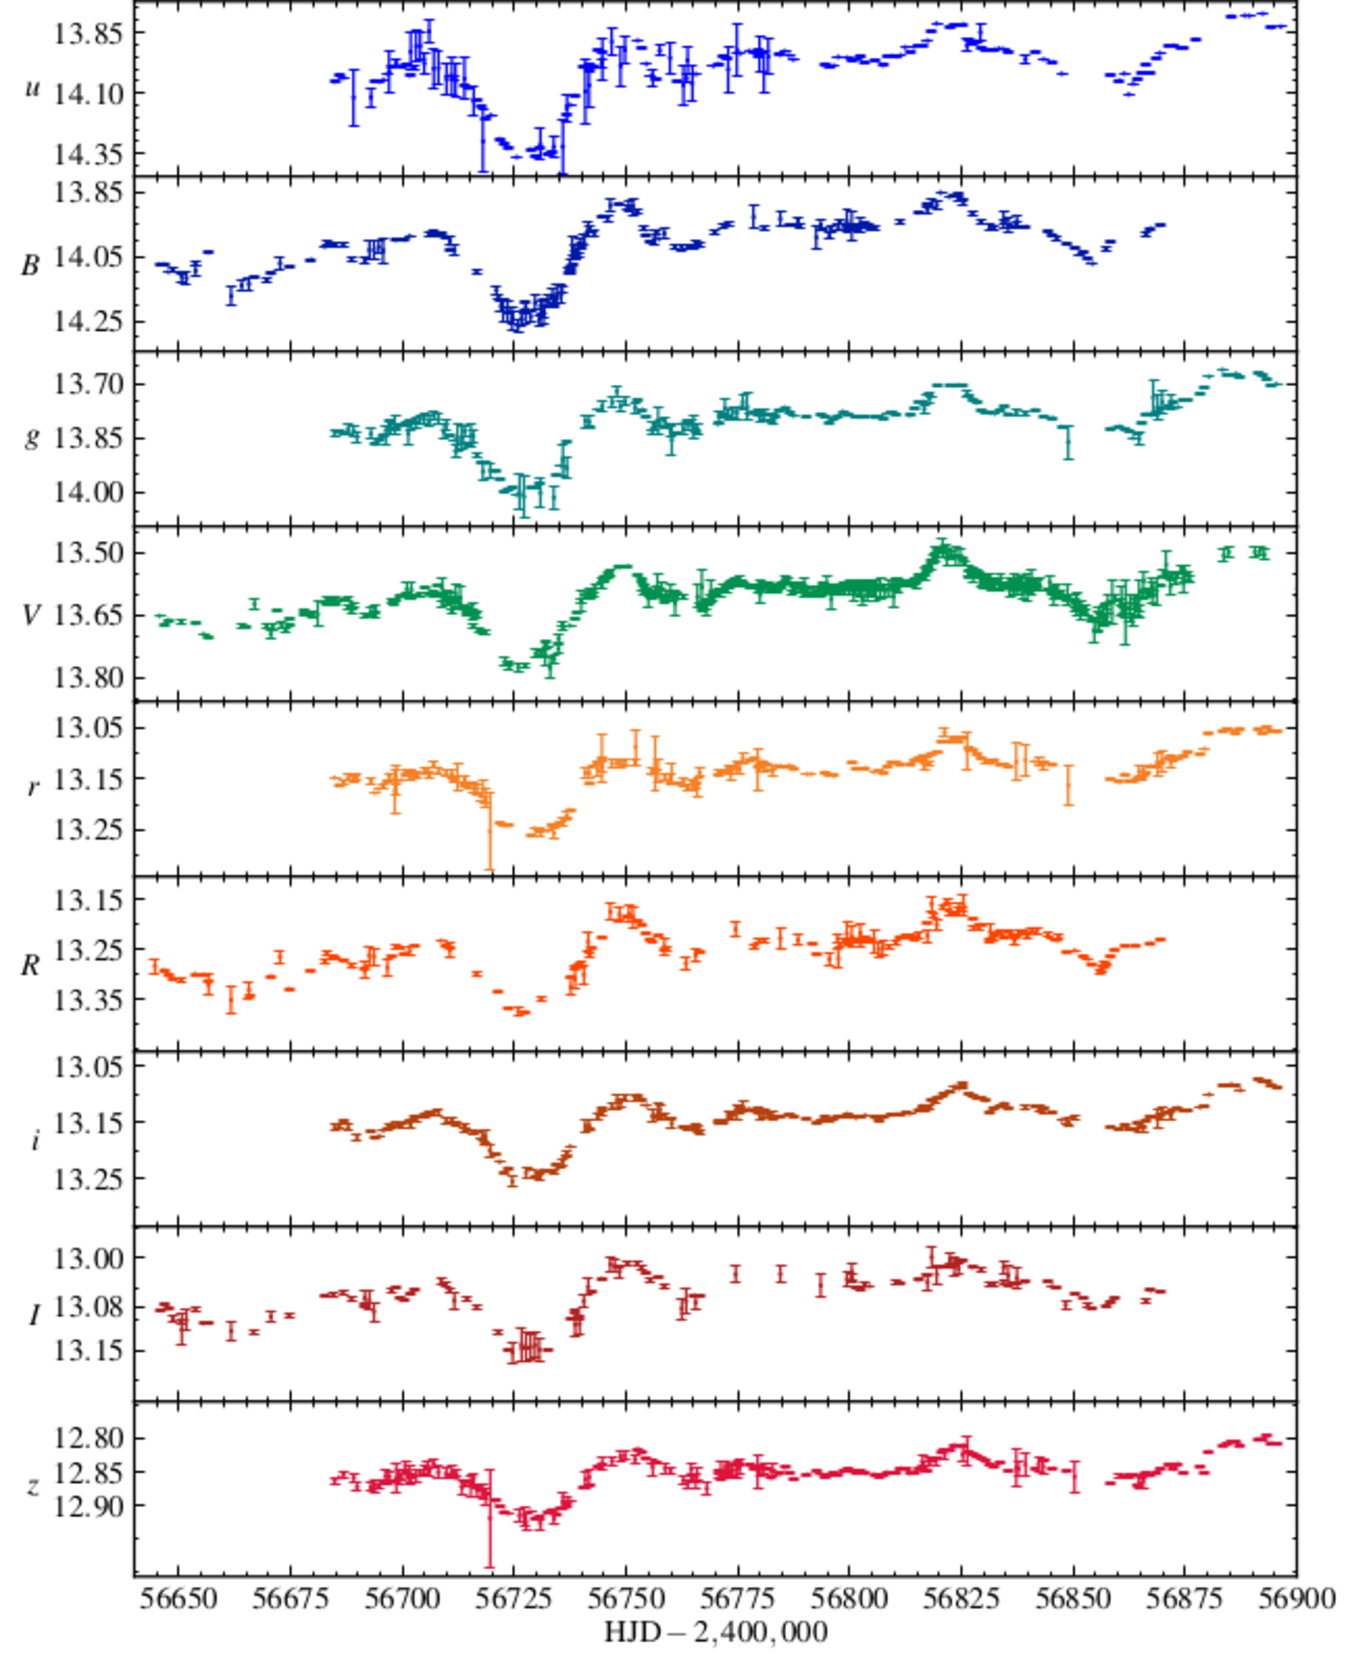
\includegraphics[width=1\linewidth]{../img/lightcurves.pdf}
    \captionof{figure}{Data published by \cite{2016ApJ...821...56F} in STORM III show strongly-variable light curves with significantly uneven sampling.}
    \label{fig:lightcurves}
\end{figure}

\begin{figure}
    \centering
    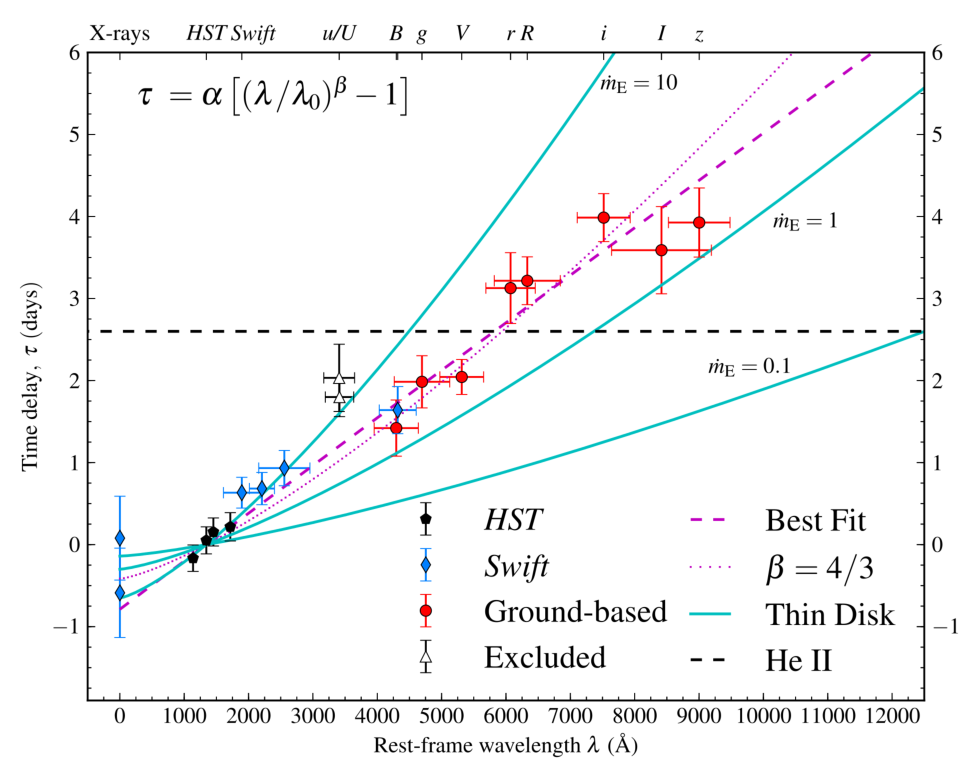
\includegraphics[width=1\textwidth]{../img/TCCF_fausnaugh.pdf}
    \captionof{figure}{Cross-correlation analysis of light curves presented by \cite{2016ApJ...821...56F} compared average time lags to AGN structure models.}
    \label{fig:cc_analysis}
\end{figure}


 The latest version as of July, 2016, of the C++ program "psdlag" developed by \cite{2013ApJ...777...24Z} is used to directly produce the PSD and cross spectra. For each wavelength, a time lag spectrum is produced by dividing the argument of the cross spectrum by $2 \pi \nu$, with $\nu$ the mean frequency for that bin.

\begin{figure}[H]
    \centering
    \begin{minipage}{.475\textwidth}
        \centering
        \includegraphics[width=1\linewidth]{../img/PSD_1367Å_{σ∊CM}.pdf}
        \captionof{figure}{Power spectral density for 1367\AA, the chosen reference band.}
        \label{fig:psd_1367}
    \end{minipage}
    \hfill
    \begin{minipage}{.475\textwidth}
        \centering
        \includegraphics[width=1\linewidth]{../img/timelag_1367Å_≺_7647Å_{σ∊CM}.pdf}
        \captionof{figure}{The time lag computed from the cross spectrum of 7647\AA and 1367\AA.}
        \label{fig:timelag_7647}
    \end{minipage}
\end{figure}


    \subsection{Errors}
	The standard errors reported for the power spectral densities and time lags are taken from the covariance matrix. This method assumes that the errors between frequency bins are not correlated, so these values represent a lower limit of the true variance. Scanning the likelihood function can provide better error estimates at the cost of computation time, as can running Monte Carlo simulations. All of these methods are built into the "psdlag" program provided by \cite{2013ApJ...777...24Z}.

    An error analysis by scanning the likelihood function was attempted, but some computational issues have yet to be resolved. Monte Carlo simulations were also attempted as a way of estimating the variability of the resultant values. Some errors obtained from this method are larger than the expected accurate values, so this analysis was also excluded. Moving forward, one of these methods will provide more accurate estimates of the variance, but the errors currently reported should be considered only a lower limit.

    \subsection{Results}
    \label{results}

    In figure \ref{fig:psd_atlas}, an atlas of the power spectral densities for all 18 reverberated bands is provided. Figure \ref{fig:timelag_atlas} provides the time lag spectrum for each band relative to 1367\AA. The reference band PSD is provided separately. Producing the time lag map is a significant step toward recovering the transfer function.

    \begin{figure}
        \centering
        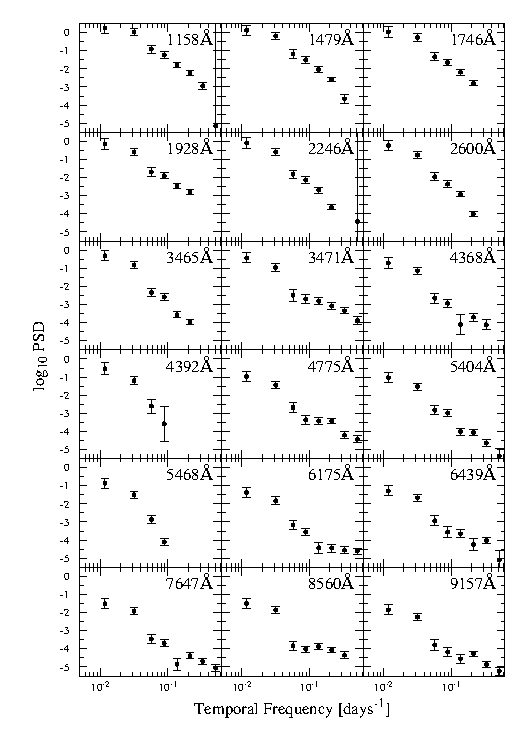
\includegraphics[width=.9\textwidth]{../img/psd_atlas.pdf}
        \caption{Power spectral densities for all observed light curves, excluding the reference curve. A decrease in variability is observed with increasing wavelength.}
        \label{fig:psd_atlas}
    \end{figure}

    \begin{figure}
        \centering
        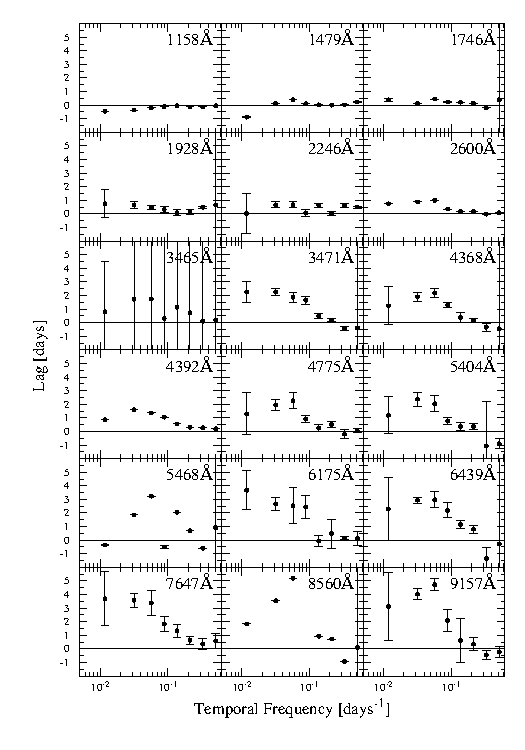
\includegraphics[width=.9\textwidth]{../img/timelag_atlas.pdf}
        \caption{Time lags for all observed light curves relative to 1367\AA. The lag increases with wavelength, as predicted for thermal reprocessing. These distributions can ultimately be used to reconstruct the transfer function.}
        \label{fig:timelag_atlas}
    \end{figure}

\section{Discussion}
The power spectral densities shown in figure \ref{fig:psd_atlas} each follow a trend with greater power at lowest frequencies, showing an approximate negative power-law distribution with increasing frequency. From inspection, it can be seen that the maximum power in the light curve decreases with increasing wavelength, meaning the UV light curves are more strongly variable than those in the near-IR. That behaviour is expected due to the blurring of reverberated emission reprocessed by the accretion disk. Better error sampling is preferred, but the trend appears clear enough to support the thermal reprocessing hypothesis. While this is apparent from inspecting the curves by eye, the exact shape of the PSD depend on the shape of the transfer function, and thus, will be important for modelling the transfer function of this system.

The time lags computed from the light curves and shown in figure \ref{fig:timelag_atlas} demonstrate an increase in magnitude in the low-to-mid frequencies as wavelength increases. As demonstrated using the tophat model, the magnitudes in this region indicate the average time lag for a particular transfer function. This indicates that the average time lag increases with wavelength, which was also seen in the time-domain cross-correlation analysis. The accretion disk geometry coupled with a decreasing temperature distribution predicts this as well. The errors computed for the time lag at 3465\AA is extremely large, but are probably no more suspicious than those errors for other wavelengths that are extremely small. As with any conclusions made regarding the PSD, better error calculations are preferred, but the trend is very strong, and this analysis appears to support the thermal reprocessing hypothesis.

The time lags follow a seemingly complex pattern with respect to frequency. Analysis of the tophat impulse response model predicted frequency-dependent time lags similar to those shown in figure \ref{fig:th_freq}. The time lag trends seen in this analysis do not resemble the saw-tooth character seen in the tophat model, so a more complex model may be a better choice for fitting the time lags. A log-Gaussian distribution is likely a good function to try next. A good fit of these curves will be required for proper recovery of the transfer function.

The analytical method developed by \cite{2013ApJ...777...24Z} applies well to the quality of data available for optical reverberation mapping. The analyses performed on these data have elucidated clear trends in the PSD and time lags. With reverberation mapping, the goal is to recover the transfer function, which encodes the geometry of the system. Recovering the time lags is a significant step toward that goal. The transfer function is within the reach of this analysis, and should be recovered in the next few steps. The error computation issues must be resolved so that any conclusions made from this analysis may be judged valid. It is our hope that this mode of analysis will be judged valid so it can be applied to datasets across the landscape of optical reverberation mapping, where considerable information awaits discovery.

%\bsp
\newcommand{\mnras}{MNRAS}
\newcommand{\apj}{ApJ}
\newcommand{\aapr}{A\&ARv}
\newcommand{\aap}{A\&A}
\newcommand{\nat}{Nature}
\newcommand{\pasp}{PASP}
\newcommand{\araa}{ARAA}
\newcommand{\ssr}{SSRv}

\bibliographystyle{mnras}
\bibliography{wsu_reu}{}



\end{document}
